\documentclass[4pt,margin=0.9in,innermargin=-1.50in,blockverticalspace=-0.001in]{tikzposter}
\geometry{paperwidth=36in,paperheight=48in}
\usepackage[utf8]{inputenc}
\usepackage{amsmath,amsfonts,amsthm,amssymb}
\usepackage{array,colortbl}
\usepackage{mathrsfs}
\usepackage{graphicx}
\usepackage{adjustbox}
\usepackage{enumitem}
\usepackage[backend=biber,style=numeric]{biblatex}
\usepackage{emory-theme,multicol}
\usepackage{tikz}
\usepackage[utf8]{inputenc}
\usepackage{longtable}
\usetikzlibrary{calc,chains,backgrounds,positioning,matrix,decorations.markings,arrows,arrows.meta}
\usepackage{pdfpages}
\usepackage{pgfplots}
\pgfplotsset{compat=1.7}
\usepackage{listings}
\usepackage{xcolor}
\usepackage{listings}
\usepackage{multirow}

\addbibresource{refs.bib}

%% For code listings
\definecolor{codegreen}{rgb}{0,0.6,0}
\definecolor{codegray}{rgb}{0.5,0.5,0.5}
\definecolor{codepurple}{rgb}{0.58,0,0.82}
\definecolor{backcolour}{rgb}{0.95,0.95,0.92}
\lstdefinestyle{mystyle}{
  backgroundcolor=\color{backcolour},   
  commentstyle=\color{codegreen},
  keywordstyle=\color{magenta},
  numberstyle=\tiny\color{codegray},
  stringstyle=\color{codepurple},
  basicstyle=\ttfamily\footnotesize,
  breakatwhitespace=false,         
  breaklines=true,                 
  captionpos=b,                    
  keepspaces=true,                 
  numbers=left,                    
  numbersep=5pt,                  
  showspaces=false,                
  showstringspaces=false,
  showtabs=false,                  
  tabsize=2
}

\lstset{
  escapeinside={{*@}{@*}}
}

    \tikzset{
      brace/.style={
        decoration={brace,amplitude=0.5cm},
        decorate
      }
    }
    \tikzstyle{ar} = [arrows={-Triangle[scale=2]}]


\usepackage{mwe} % for placeholder images

\hyphenpenalty=5000

\usepackage{xspace}

% Custom Macros
\newcommand{\MiddFS}[2]{#1{M}#2{iddFS }#1{i}#2{s'nt mi}#1{d}#2{\quad \quad}#1{d}#2{\quad \quad}#1{F}#2{ile\quad}#1{S}} % #1 large; #2 small
\newcommand{\middfs}{\texttt{middfs}}
\newcommand{\rc}{\rowcolor}
\newcommand{\ZC}{{\textsc{ZC}}\xspace}

% set theme parameters
\tikzposterlatexaffectionproofoff
\usetheme{EmoryTheme}
\usecolorstyle{EmoryStyle}

\title{\rm \ZC: a C Compiler for the (e)Z80}
\author{\vspace{1cm} Nicholas Mosier '20 \\ \vspace{1cm} \small \texttt{https://github.com/nmosier/zc.git}}
\titlegraphic{\includegraphics[width=0.2\textwidth]{mdl_master_left_blue.png}}

% begin document
\begin{document}
\maketitle

\centering

\begin{columns}
  \column{0.5}
  \block{Introduction \& Motivation}{
%    The Zilog Z80 is an 8-bit microprocessor that used to be ubiquitious in personal computing and arcade gaming in the 1970-80's. We introduce ZC, a C compiler for the eZ80 variant of the Z, is still used to this day in Texas Instrument's TI-83/84+ graphing calculators. More recently, the eZ80 processor, introduced in the early 2000's, features a minor, backwards-compatible update to the original Z80 ISA, and is used in the TI's higher-end calculators, e.g. the TI-84+ CE. TI calculator programmers (including me), 

    \begin{minipage}{0.55\linewidth}
    \innerblock{Motivation}{
      \begin{itemize}
      \item Z80 \& eZ80 still used in Texas Instruments graphing calculators
      \item Large code size output of existing C compilers targeting the eZ80
      \item High-performance C compiler essential for large (e)Z80 projects
      \end{itemize}
    }
    \end{minipage}
    \begin{minipage}{0.35\linewidth}
    \innerblock{The Zilog Z80 \& eZ80}{
      \begin{itemize}
      \item 8-bit CISC mircoprocessor
      \item Accumulator machine model
      \item 16-/24-bit register pairs \& addresses
      \end{itemize}
    }
  \end{minipage}

  Due to shortcomings in existing compilers, I wrote \ZC,
  a C compiler for the eZ80 architecture that optimizes for code size.
  }

  \block{Compiler Anatomy}{
    \begin{center}
    \begin{minipage}{0.95\linewidth}
    \ZC accepts a C source file as input and produces (e)Z80 assembly as output.
    The \ZC compiler frontend parses the input into an
    {\it abstract syntax tree} (AST) and annotates it,% with type information,
    while the backend translates the AST into a control flow
    graph and performs optimizations.
  \end{minipage}
  \end{center}
    \vspace{1cm}
    
    \begin{minipage}{0.5\linewidth}
    \innerblock{Frontend}{
      {\bf Lexer and parser:}
      \begin{itemize}
      \item Parses input C program into AST
      \item Implemented using {\tt flex} and {\tt bison} tools
      \end{itemize}
      %The lexer and parser, written for the {\tt flex} and {\tt bison} tools, implement the C grammar and define the rules for constructing an AST representing the input program.

      {\bf Semantic Analysis:}
      \begin{itemize}
      \item Infers types of AST expressions
      \item Checks semantic validity
      \item Resolve user-defined types such as {\tt typedef}s
      \end{itemize}
      %ZC infers the types of expressions in the AST, resolves user-defined types such as {\tt struct}s and {\tt typedef}s, and checks semantic validity of the program.
    }
    \end{minipage}
    \begin{minipage}{0.5\linewidth}
    \innerblock{Backend}{
      {\bf Code Generation:}
      \begin{itemize}
      \item Outputs control flow graph of basic blocks
      \item Blocks contain symbolic (e)Z80 instructions
      \item Generates function activation record layout
      \end{itemize}
      %For each function, ZC generates a control flow diagram of basic blocks containing symbolic (e)Z80 instructions and determines an activation record layout.

      {\bf Register allocation: }
      \begin{itemize}
      \item Assigns registers to variables in basic blocks
      \item Stack- and frame-spill when necessary
      \end{itemize}
    }
    \end{minipage}

    
    \begin{tikzfigure}
      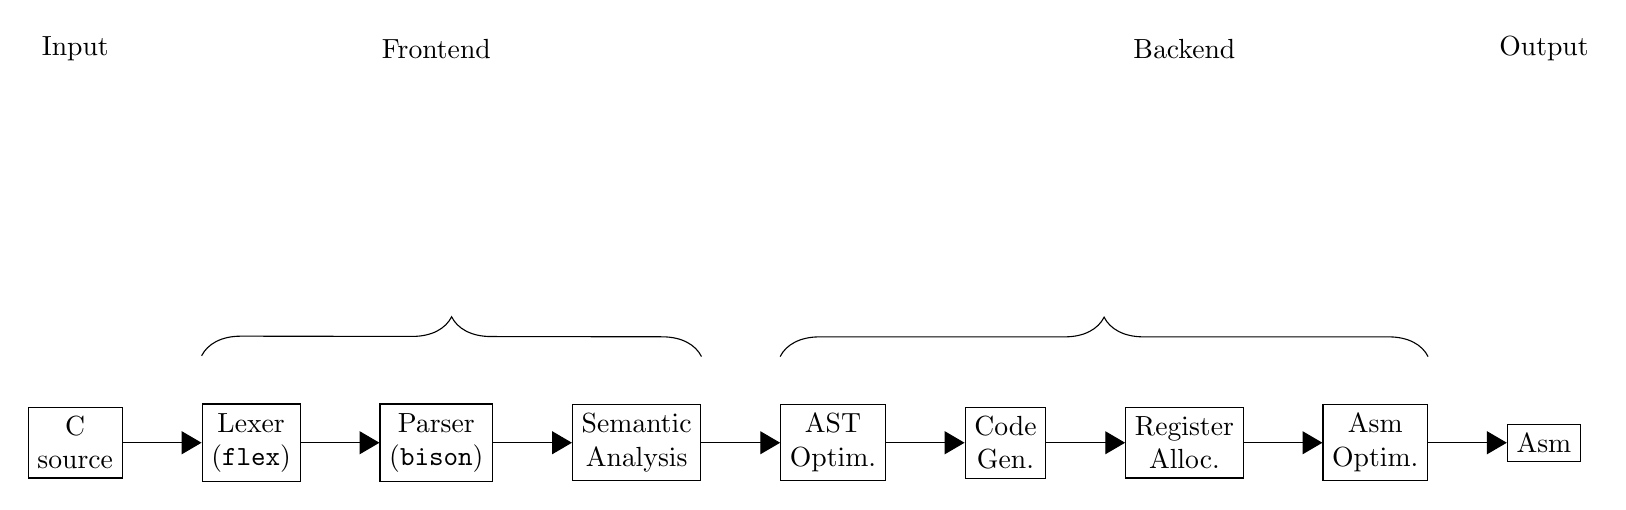
\begin{tikzpicture}[
        start chain,
        node distance=1cm,
        zc/.style={draw,on chain,align=center,join=by ar},
        zcl/.style={node distance=5cm},
        zcb/.style={brace,decoration={raise=4ex}},
        ]

        \node[zc] (src) {C \\ source};
        \node[zc] (lexer) {Lexer \\ ({\tt flex})};
        \node[zc] (parser) {Parser \\ ({\tt bison})};
        \node[zc] (semant) {Semantic \\ Analysis};
        \node[zc] (astopt) {AST \\ Optim.};
        \node[zc] {Code \\ Gen.};
        \node[zc] (ralloc) {Register \\ Alloc.};
        \node[zc] (asmopt) {Asm \\ Optim.};
        \node[zc] (asm) {Asm};

        \node[zcl] (in) [above of=src] {Input};
        \node[zcl] (out) [above of=asm] {Output};

        \node[zcl] (frontend) [above of=parser] {Frontend};
        \node[zcl] (backend) [above of=ralloc] {Backend};

        \draw[zcb] (lexer.north west) -- (semant.north east);
        \draw[zcb] (astopt.north west) -- (asmopt.north east);
        
      \end{tikzpicture}
      
    \end{tikzfigure}

  }

  \block{Register Allocation} {
    Two approaches to code generation are the {\it stack machine} model and the
    {\it register allocator} model.
    \ZC performs register allocation in order to minimize code size.
    % While implementing a stack machine is simpler, implementing a register allocator better utilizes resources and exposes code to more optimizations.
    
    % Stack Machine vs. Register Allocation
    \begin{minipage}{0.5\linewidth}
      \innerblock{Stack Machine}{
        \begin{itemize}
        \item Pushes variables onto the stack and pops them off when ready for use
        \item Easy to implement
        \item \ZC's first code generator used a stack machine
        \end{itemize}
        % A stack-machine compiler pushes intermediate values onto the stack and pops them off when they are ready to be used. A stack machine is easy to implement; the first version of ZC's code generator was a stack machine.
      }
    \end{minipage}
    \begin{minipage}{0.5\linewidth}
      \innerblock{Register Allocation}{
        \begin{itemize}
        \item Stores variables in registers, not on the stack
        \item {\it Spills} variables into memory if all registers are in use
        \item Exposes code to more optimizations
        \end{itemize}
        %A compiler with a register allocator stores intermediate values into registers rather than pushing them onto the stack. However, there are often more intermediate values than there are physical registers. For example, the (e)Z80 has {\bf 7 single-byte registers} but only {\bf 3 allocatable multi-byte registers}. When intermediate values exceed physical registers in number, those values must be \textit{spilled} into memory.
      }
    \end{minipage}
    
    \begin{minipage}{0.5\linewidth}
      \innerblock{(e)Z80 Restrictions}{
        \begin{itemize}
        \item Only 3 allocatable multibyte registers
        \item Instruction set biased towards accumulator
        \item Most register allocation algorithms assume all registers are equal
        \item \ZC implements specialized algorithm accounting for mixture of fixed registers and unbound variables
        \end{itemize}
        % The (e)Z80's instruction set is accumulator-based: most operations aside from moves require the destination and first operand to be the byte register {\tt a} or the multibyte register {\tt hl}. Traditional register allocation does not account for this bias, so our ZC compiler implements a specialized register allocation algorithm that accounts for some operands being fixed registers and others being unbound variables.
    }
    \end{minipage}
    \begin{minipage}{0.5\linewidth}
      \innerblock{Frame vs. Stack Spilling in \ZC}{
        \ZC spills variables in two ways.

        \begin{itemize}
          \item {\bf Frame spilling}: {\it Costly but versatile}. 
        Most compilers perform frame spilling, i.e. spill variables to the activation record. However, memory access through the frame pointer register {\tt ix} is costly in (e)Z80.
        \item {\bf Stack spilling}: {\it Cheap but restrictive}.
          To stack spill, i.e. push/pop variables to/from the stack, is more efficient in (e)Z80. Stack spilling is a novel feature of \ZC's register allocator.
        \end{itemize}
        
        
        %Most compilers use {\it frame spilling}, i.e. spill intermediate values to the activation record. However, accessing memory through the frame pointer register {\tt ix} is costly in (e)Z80; {\it stack spilling}, i.e. to push/pop intermediate values to/from the stack, is more efficient. Stack spilling is {\bf cheap but restrictive}; frame spilling is {\bf costly but versatile}.
    }
    \end{minipage}

    \begin{tikzfigure}
    {\tt
      \begin{tabular}{|>{\bf}ll|>{\bf}ll|>{\bf}ll|}\hline
        \multicolumn{2}{|c|}{\hspace{0.5cm}\bf Stack Machine \hspace{0.5cm}}
        & \multicolumn{4}{|c|}{\bf Register Allocation} \\
        & & \multicolumn{2}{c}{\rm Before} & \multicolumn{2}{c|}{\rm After}
        \\\hline
        ld & a,(ix+7) & ld & {\it vb4} ,(ix+7) & ld & a,(ix+7) \\
        push & af & & & & \\
        ld & a,97 & ld & {\it vb5},97 & ld & l,97 \\
        pop & bc & ld & a,{\it vb4} & ld & a,a \\
        cp & a,b & cp & a,{\it vb5} & cp & a,l \\
        \hline
      \end{tabular}
    }
    \end{tikzfigure}

    
  }
    
  
  \column{0.5}

  
  \block{Performance}{
    I tested \ZC on four programs against a reference compiler,
    Zilog's C compiler for the eZ80 \cite{ez80cc}.
    On average, \ZC's performance is comparable to the reference compiler,
    though each compiler produces more compact code in a subset of programs.
    These results are encouraging, since there are many unimplemented
    optimizations for future work on \ZC.
    \begin{tikzfigure}
      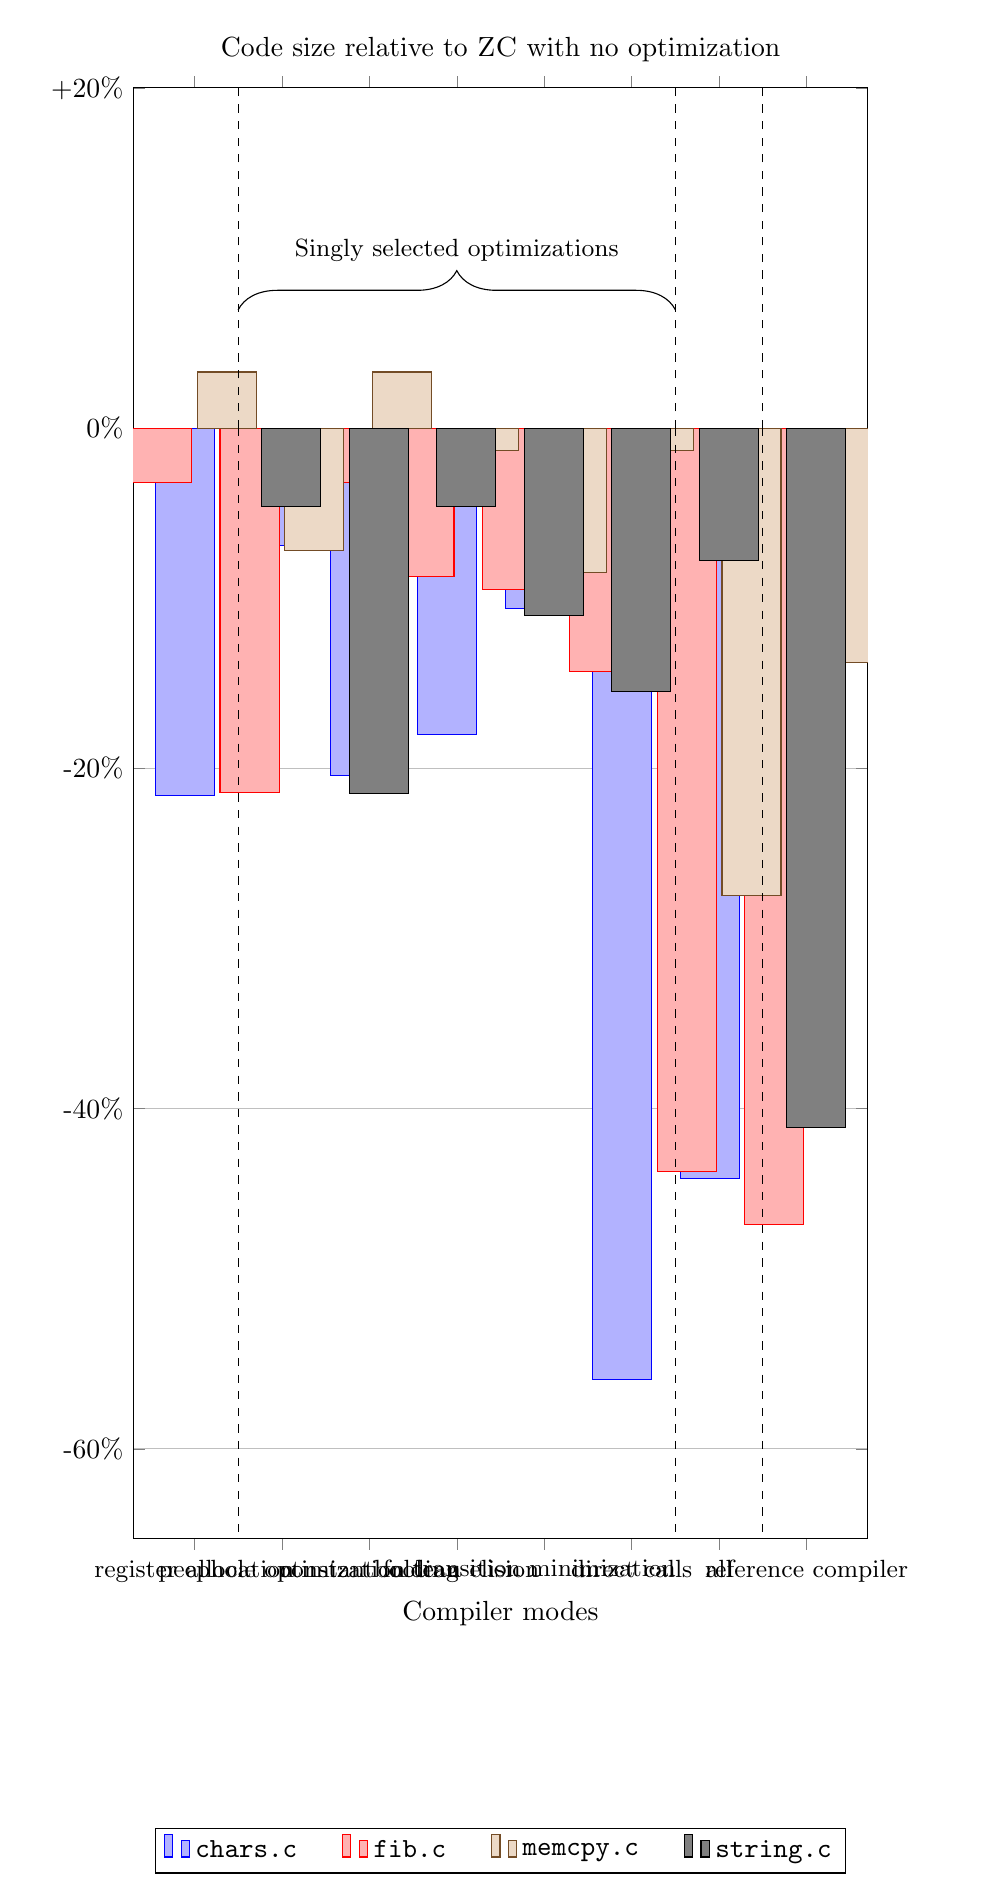
\begin{tikzpicture}
        \begin{axis}[
          width=0.9\linewidth,
          height=20cm,
          ybar,
          symbolic x coords={register allocation, peephole optimization, constant folding, boolean elision, transition minimization, direct calls, all, reference compiler},
          enlarge x limits=true,
          xtick=data,
          ytick={0,20,-20,-40,-60},
          yticklabels={0\%,+20\%,-20\%,-40\%,-60\%},
          ymajorgrids=true,
          ymax=20,
          %ylabel={Percentage (\%)},
          xlabel={Compiler modes},
          legend style={
            at={(0.5, -0.2)},
            anchor=north,
            legend columns=-1,
            /tikz/every even column/.append style={column sep=0.5cm}
          },
          x tick label style={font=\small, text width=4cm, align=center},
          bar width=0.75cm,
          title style={align=center},
          title={Code size relative to \ZC with no optimization}
          ]

          % chars.c
          \addplot coordinates {
            (register allocation,-4.9)
            (peephole optimization,-21.6)
            (constant folding,-6.9)
            (boolean elision,-20.4)
            (transition minimization,-18.0)
            (direct calls,-10.6)
            (all,-55.9)
            (reference compiler,-44.1)
          };
          

          % fib.c
          \addplot coordinates {
            (register allocation,-3.2)
            (peephole optimization,-21.4)
            (constant folding,-3.2)
            (boolean elision,-8.7)
            (transition minimization,-9.5)
            (direct calls,-14.3)
            (all,-43.7)
            (reference compiler,-46.8)
          };

          % memcpy.c
          \addplot coordinates {
            (register allocation,3.3)
            (peephole optimization,-7.2)
            (constant folding,3.3)
            (boolean elision,-1.3)
            (transition minimization,-8.5)
            (direct calls,-1.3)
            (all,-27.5)
            (reference compiler,-13.8)
          };

          % string.c
          \addplot coordinates {
            (register allocation,-4.6)
            (peephole optimization,-21.5)
            (constant folding,-4.6)
            (boolean elision,-11)
            (transition minimization,-15.5)
            (direct calls,-7.8)
            (all,-41.1)
            (reference compiler,-57.5)
          };

          \legend{\texttt{chars.c}, \texttt{fib.c}, \texttt{memcpy.c},
            \texttt{string.c}}

          \path(axis cs:all,0) -- coordinate (m) (axis cs:reference compiler,0);
          \draw[dashed] (m) -- (current axis.south -| m);
          \draw[dashed] (m) -- (current axis.north -| m);

          \path(axis cs:register allocation,0) -- coordinate (n) (axis cs:peephole optimization,0);
          \draw[dashed] (n) -- (current axis.south -| n);
          \draw[dashed] (n) -- (current axis.north -| n);          

          \path(axis cs:direct calls,0) -- coordinate (o) (axis cs:all,0);
          \draw[dashed] (o) -- (current axis.south -| o);
          \draw[dashed] (o) -- (current axis.north -| o);

          \draw[decoration={brace,raise=1.5cm,amplitude=0.5cm},decorate]
          (n) -- node[above=2cm] {\small Singly selected optimizations} (o);

        \end{axis}
      \end{tikzpicture}
    \end{tikzfigure}

    \innerblock{}{
      \begin{tikzfigure}
        \centering
        \begin{tabular}{|c|c|c|c|c|}\hline
          & {\tt chars.c} & {\tt fib.c} & {\tt memcpy.c} & {\tt string.c} \\\hline
          {(stack machine)} & (\textcolor{red}{245}) & (\textcolor{red}{126}) & (305) & (\textcolor{red}{219}) \\\hline
          register allocation & 233 & 122 & 313 & 208 \\\hline
          peephole optimization & 192 & 99 & 283 & 173 \\\hline
          constant folding & 228 & 122 & \color{red} 315 & 208 \\\hline
          boolean elision & 195 & 115 & 301 & 194 \\\hline
          transition minimization & 201 & 114 & 279 & 176 \\\hline
          direct calls & 219 & 108 & 301 & 20 \\\hline
          {\bf all} & {\bf 108} & {71} & {\bf 221} & {122} \\\hline
          {\it reference compiler} & {\it 137} & {\bf \textit{67}} & {\it 263} & {\bf\textit{93}} \\\hline
        \end{tabular}

      \end{tikzfigure}
    }
  }

  \block{Optimizations Overview}{

    \begin{multicols}{2}
    \begin{itemize}
    \item {\bf Peephole optimization:} find suboptimal instruction patterns in a
      sliding window and replace with shorter equivalent.
    \item {\bf Constant folding:} compute constant expressions at compile-time.
    \item {\bf Boolean elision:} skip producing boolean values in registers; use the flag states directly.
    \item {\bf Transition minimization:} emit basic blocks in such an order that jump transitions can fall through to the destination block.
    \item {\bf Direct calls:} when calling a constant function expression, call it directly (rather than loading the address into a register).
    \end{itemize}
    \end{multicols}
    
  }
  
  \block{Optimization Examples}{
    \innerblock{Peephole}{
      \begin{minipage}{0.33\linewidth}
        \centering
        Useless pushes \& pops \\
        \vspace{0.5cm}
        \tt
        \begin{tabular}{|>{\bf}ll|c|>{\bf}ll|}\cline{1-2}\cline{4-5}
          or   & a,a   &\multirow{6}{*}{$\rightarrow$}& or & a,a \\
          sbc  & hl,hl && sbc & hl,hl \\
          ld   & l,a   && ld & l,a \\
          \color{red} push & \color{red} hl &&& \\
          \color{red} pop  & \color{red} hl &&& \\
          jp & lbl0 && jp & lbl0 \\
          \cline{1-2}\cline{4-5}
        \end{tabular}
      \end{minipage}
      \begin{minipage}{0.33\linewidth}
        \centering
        Frame unsetting with \\ no local variables \\
        \vspace{0.5cm}
        \tt
        \begin{tabular}{|>{\bf}ll|c|>{\bf}ll|}\cline{1-2}\cline{4-5}
          \color{red} lea & \color{red} ix,ix+0 & \multirow{4}{*}{$\rightarrow$} && \\
          \color{red} ld & \color{red} sp,ix &&& \\
          pop & ix && pop & ix \\
          ret &&& ret & \\
          \cline{1-2}\cline{4-5}
        \end{tabular}
      \end{minipage}%
      \begin{minipage}{0.33\linewidth}
        \centering        
        Loading zero becomes \\ self-subtraction \\
        \vspace{0.5cm}
        \tt
        \begin{tabular}{|>{\bf}ll|c|>{\bf}ll|}\cline{1-2}\cline{4-5}
          \color{red} ld & \color{red} a,a & \multirow{3}{*}{$\rightarrow$} & \color{green} or & \color{green} a,a \\
          \color{red} ld & \color{red} hl,0 && \color{green} sbc & \color{green} hl,hl \\
          ld & l,a && ld & l,a \\
          \cline{1-2}\cline{4-5}
        \end{tabular}
      \end{minipage}
    }

    \begin{minipage}{0.5\linewidth}
    \innerblock{Boolean Elision}{
      \tt
      \centering
        \begin{tabular}{|>{\bf}ll|c|>{\bf}ll|}\cline{1-2}\cline{4-5}
          ld & l,`A' & \multirow{7}{*}{$\rightarrow$} & ld & l,`A' \\
          cp & a,l && cp & a,l \\
          \color{red} sbc & \color{red} a,a &&& \\
          \color{red} inc & \color{red} a &&& \\
          \color{red} or & \color{red} a,a &&& \\
          \color{red} jp & \color{red} nz,label0 && \color{green} jp & \color{green} nc,label0 \\
          \color{red} jp & \color{red} z,label1 && \color{green} jp & \color{green} c,label1 \\
          \cline{1-2}\cline{4-5}
        \end{tabular}
      }
    \end{minipage}%
    \begin{minipage}{0.5\linewidth}
      \innerblock{Constant Folding}{
        \tt
        \centering
        \begin{tabular}{|>{\bf}ll|c|>{\bf}ll|}\cline{1-2}\cline{4-5}
          ld & l,(ix+7) & \multirow{5}{*}{$\rightarrow$} & ld & l,(ix+7) \\
          ld & a,\color{red}`A' && ld & a,\color{green}-32 \\
          \color{red} ld & \color{red} h,`a' &&& \\
          \color{red} sub & \color{red} a,h &&& \\
          add & a,l && add & a,l \\
          \cline{1-2}\cline{4-5}
        \end{tabular}
      }
      \end{minipage}
}

%\block{Future Work}{
%\begin{itemize}
 %   \item Global register allocation (ZC currently only does local, i.e. basic block, register allocation)
      
  %  \end{itemize}
  %}
\end{columns}

\block{}{
  \hrule
  \begin{minipage}{0.5\linewidth}
    \innerblock{Acknowledgements}{
      Thanks to Professor Michael Linderman for adivising this project
      during Winter 2020.
    }
  \end{minipage}
  \begin{minipage}{0.5\linewidth}
    \innerblock{References}{
      \begin{footnotesize}
        \printbibliography[heading=none]
        \nocite{*}
      \end{footnotesize}
    }
  \end{minipage}
}

\end{document}
